\subsection{A Clustering-Based Method for Automatic Educational Video Recommendation Using Deep Face-Features of Actors}

In this second application we used \emph{video face clustering} for recommending videos that share the presence of the same actors. %%
This work aimed at recommending educational video content based on actors' presence.
%%
To do that, we perform \emph{video face clustering} in all videos from a certain dataset and calculate their centroids.
%%
By the end of this step, we have each video in the dataset represented by its centroids where, ideally, each centroid represents an actor present in the video.


Given these centroids, we perform a clustering step for creating a relationship between videos that share the presence of the same actors.
%%
By doing that, we group centroids from the same actor that are in different videos. For instance, in Figure \ref{fig:video_recommendation}, one can see that the \emph{purple actor} is present in both Videos 1 and 2, while the \emph{orange actor} is present in both Videos 2 and n. 
%%
By the end of this step, we have the group $L$ of actors present in the dataset of videos $V$, and we can also denote $L_v$ as the group of actors present in video $v$.

\begin{figure*}[!ht]
  \centering
  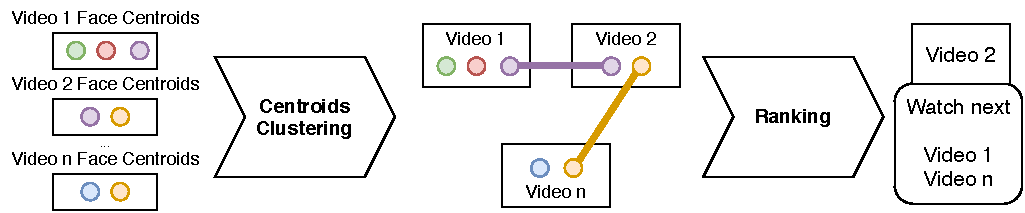
\includegraphics[width=0.8\linewidth]{img/ism/video_recommendation.pdf}
  \caption{Video Recommendation process.}
  \label{fig:video_recommendation}
\end{figure*}

Finally, we rank the recommended videos based on the amount of time the referenced actors were present.
%%
For doing that, we compute a similarity score using the presence of the actors in the current video and the presence of these same actors in the other video.
%%
Let $p_{l,v}$ denote the percentage of frames in which the actor $l \in L_v$ is present in video $v \in V$. For each video $v \in V$ and $u \in V-v$ we compute a score of similarity $S_{v,u}$.

\vspace{-1em}
\begin{equation}
  S_{v,u} = \sum_{l~\in~L_v}{p_{l,v}\cdot{p_{l,u}}}
\end{equation}

Using this score for each video $v$ we compute a ranking $R_{v}$ where $R_{v,i}$ denotes the \emph{i-greatest} $S_v$ and $R_{v,i}\ge~R_{v,i+1}$ for all $i~\in~1...n_v$, where $n_v$ is the number of videos $u$ in which $S_{v,u}>~0$. 
%%
In this way, the more actors a video have in common with the reference video, and the more time these actors are present in both videos, the higher the video is positioned in the ranking of the reference video.  
%%
By the end of this pipeline, we have a ranking of recommended videos for each video in the dataset.
%%
It is important to notice that our method is unsupervised and does not require the information of the actors in advance.
%%
Consequently, we do not store any information regarding the identity of the actors, respecting their privacy.
%%
A particular feature of this approach is that it can be done without supervision, allowing for new videos to be automatically analyzed

We evaluate our approach based on the relevance of the videos recommended. 
%%
In our evaluation, we constructed a dataset of educational videos extracted from YouTube.
%%
Details about this evaluation will be described in our dissertation. 
%%
This application has also been published at a relevant multimedia conference~\cite{mendes2020ISM}.